\documentclass[Softwaredesign/Softwaredesign_main.tex]{subfiles}

\begin{document}


\textbf{Brug af QT Creator freamwork}
I QT Creator frameworker er alt baseret på, at der til at starte med er et "MainWindow" objekt.  Dette objekt bliver instantiereret øjeblikket programmet bliver startet op.  MainWindow arver fra typen "QMainWindow" , som indeholder en masse funktionalitet,  til at manipulere indholdet af Mainwindow: Widgets, Labels osv.  Dette kan gøres gennem en UI::MainWindow pointer, kaldt ui, som lagres i MainWindow objektet. Et eksempel på brug af QMainWindow funktionalitet gennem denne pointer kunne være:
\begin{verbatim}
ui->infotext->setText("EksempelTekst");
\end{verbatim}
Den før nævnte  QMainWindow type arver også, fra typen QWigdet. Denne type indeholder også en masse funktionalitet. Forskellen melllem QMainWindow og Qwidget er; QMainWindow styre indeholdet af vinduet, men QWidget styre selve vinduet. Det kunne være f.eks.  om vinduet skal være maksimeret eller minimeret, titlen på vinduer osv. 
\begin{verbatim}
window->setWindowTitle("Eksempel title");
\end{verbatim}
Til sidst arver QWidget også fra QObject, her igen er der meget funktionalitet. Denne her klasse indeholder dog funktionalitet for en masse baggrunds indhold. Det kunne være f.eks.: oprettelse af tråde, oprettelse af timers, oprettelse af forbindelser mellem QWidgets osv. Denne funktionallitet bruges ikke indenfor Display delen af RPI applikationen, så her er eksempel ikke nødvendigt. 

\begin{figure}[H]
    \centering
    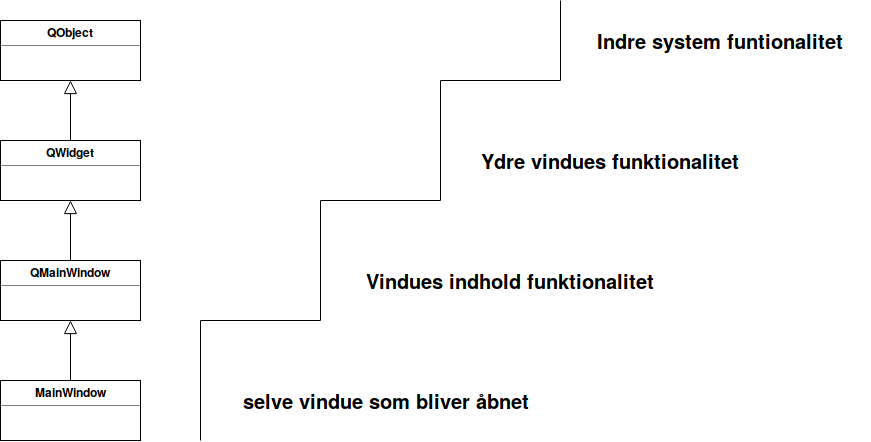
\includegraphics[scale=0.5]{Softwaredesign/GUI/Pictures/Brug_af_Framework.png}
    \caption{Forsimplet klasse diagram over Framework strukturen, vist ved siden af er en pyramide struktur, som viser funktionalitet hierarkiet}
    \label{fig:brug_af_framework}
\end{figure}

\end{document}